\documentclass[11pt]{article}
\usepackage[a4paper,margin=1in]{geometry}
\usepackage{amsmath,amssymb,amsthm}
\usepackage{tikz}
\usetikzlibrary{arrows.meta,calc}
\usepackage{xcolor}
\usepackage{booktabs}
\usepackage[hidelinks]{hyperref}
\hypersetup{pdftitle={Catching the centroid},pdfauthor={Vamshi Jandhyala}}
\setlength{\parskip}{0.4em}
\setlength{\parindent}{0pt}

\newtheorem{theorem}{Theorem}
\newtheorem{proposition}{Proposition}
\newtheorem{lemma}{Lemma}
\theoremstyle{remark}
\newtheorem*{remark}{Remark}

\definecolor{inkblue}{RGB}{40,76,105}
\definecolor{softblue}{RGB}{226,235,243}
\definecolor{rust}{RGB}{153,70,45}

\newcommand{\ro}{\rho_{\mathrm o}}
\newcommand{\abs}[1]{\left|#1\right|}

\title{Catching the centroid}
\author{Vamshi Jandhyala}
\date{}

\begin{document}
\maketitle
\vspace{-2em}

\begin{abstract}
Choose two random points in a planar convex region and draw the circle that has them as the ends of a
diameter. How likely is the circle to contain the centroid? For a disc or a square the answer is exactly
$1/2$, for an equilateral triangle it is $1/3+\tfrac16\ln 3\approx 0.5164$, and the triangle is
conjectured to be the best possible shape. This note shows that the excess over $1/2$ comes entirely from
the asymmetry of the region about its centroid, and that it is at most the product of two classical
measures of asymmetry. With the theorems of Gr\"unbaum and of Stewart this gives the bound
$14/27\approx 0.5185$ for every convex region. For regions whose boundary crosses its reflection
through the centroid six times, which includes every region close to a triangle, Stewart's theorem
has a three-line proof from Gr\"unbaum's. The arguments have been checked in the Lean proof
assistant, with the two classical theorems as stated inputs.
\end{abstract}

\section{A circle on a random diameter}

Let $K$ be a convex region in the plane with centroid $G$. Pick two points $X$ and $Y$ independently and
uniformly in $K$, and draw the circle with diameter $XY$. Write $P(K)$ for the probability that this
circle contains $G$.

Stop and try two cases before reading on. When $K$ is a square, what is $P(K)$? And when $K$ is an
equilateral triangle, is $P(K)$ larger or smaller?

The tool for both is a theorem of Euclid (III.31): $G$ lies inside the circle on $XY$ exactly when the
angle $XGY$ is at least a right angle. Hold $X$ fixed. The good positions for $Y$ are then the points of
$K$ on the far side of the line through $G$ perpendicular to $GX$, the shaded region in
Figure~\ref{fig:setup}. For a square every line through the centre cuts it into two halves of equal area,
so whatever $X$ is, $Y$ succeeds with probability exactly $1/2$, and $P(\text{square})=1/2$.

\begin{figure}[ht]
\centering
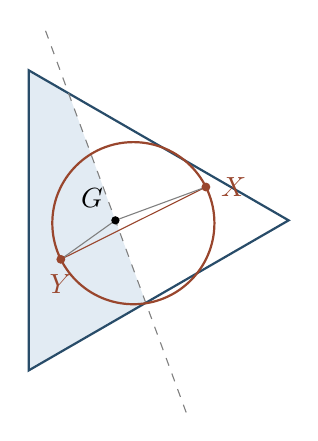
\begin{tikzpicture}[scale=1]
\draw[fill=softblue,draw=none] (-0.5944,1.6133) -- (-1.1000,1.9053) -- (-1.1000,-1.9053) -- (0.3859,-1.0474) -- cycle;
\draw[thick,inkblue] (2.2000,0.0000) -- (-1.1000,1.9053) -- (-1.1000,-1.9053) -- cycle;
\draw[gray,dashed] (0.899,-2.440) -- (-0.899,2.440);
\draw[rust,thick] (0.2282,-0.0357) circle (1.0294);
\draw[rust] (1.1495,0.4235) -- (-0.6930,-0.4950);
\draw[gray] (0,0) -- (1.1495,0.4235) (0,0) -- (-0.6930,-0.4950);
\fill (0,0) circle (1.5pt) node[above left=1pt] {$G$};
\fill[rust] (1.1495,0.4235) circle (1.6pt) node[right=2pt] {$X$};
\fill[rust] (-0.6930,-0.4950) circle (1.6pt) node[below=2pt] {$Y$};
\end{tikzpicture}

\caption{Once $X$ is chosen, the circle on $XY$ contains the centroid $G$ exactly when $Y$ lies in the
shaded part of $K$, beyond the line through $G$ perpendicular to $GX$.}
\label{fig:setup}
\end{figure}

For the equilateral triangle the shaded part is not always half. When $X$ lies towards a vertex, the
far side contains the opposite edge and holds more than half the area; when $X$ lies towards an edge,
the far side holds less. Dan, who asked the question on Mathematics Stack Exchange~\cite{MSE}, computed
\[
P(\text{equilateral triangle}) = \frac13+\frac{\ln 3}{6} \approx 0.516435,
\]
so the triangle beats the square, and asked which convex shape does best. The answers there
conjecture that the equilateral triangle is optimal, prove it among regular polygons, and observe that
without convexity the probability can approach $2/3$. The conjecture is still open.

The question is worth a look for a structural reason. Most extremal problems about random points in a
convex region are affine invariant, and there the triangle often wins by a standard argument (shadow
systems, Section~\ref{sec:left}). Here the angle at $G$ is not affine invariant, different triangles give
different values (Table~\ref{tab:values}), and the standard argument fails. Something has to measure
how far a region is from being symmetric about its centroid.

The main result of this note is a bound within $0.0021$ of the conjectured value.

\begin{theorem}\label{thm:A}
For every planar convex region $K$, $\abs{P(K)-\tfrac12}\le \tfrac1{54}$; in particular
$P(K)\le 14/27\approx 0.5185$.
\end{theorem}

It comes from one estimate, Proposition~\ref{prop:product}, which bounds $P(K)-\tfrac12$ by the product
of two measures of asymmetry, each controlled by a classical theorem about the centroid. The second of
these, Stewart's, is less often quoted than Gr\"unbaum's; Section~\ref{sec:near} gives a short proof of it
for regions close to a triangle. Section~\ref{sec:left} explains why $14/27$ is not the end of the
story.

\section{From points to directions}\label{sec:directions}

Put $G$ at the origin and use polar coordinates. The boundary of $K$ is $r=r(\theta)$, where $r(\theta)$ is
the distance from $G$ to the boundary in the direction $\theta$. A thin sector of angle $d\theta$ has area
$\tfrac12 r(\theta)^2\,d\theta$, so the direction of a uniform random point of $K$ has density
\[
\rho(\theta)=\frac{r(\theta)^2}{2\abs{K}},\qquad \int_0^{2\pi}\rho(\theta)\,d\theta=1 .
\]
The good half-plane for $X$ in direction $\theta$ consists of the directions $\varphi$ that make an angle of
at least $90^\circ$ with $\theta$, so its share of the area is
\[
a(\theta)=\int_{\theta+\pi/2}^{\theta+3\pi/2}\rho(\varphi)\,d\varphi .
\]
Averaging over the direction of $X$ gives the formula everything else rests on:
\begin{equation}\label{eq:P}
P(K)=\int_0^{2\pi}\rho(\theta)\,a(\theta)\,d\theta .
\end{equation}
Read it as: the chance that $X$ points in direction $\theta$, times the chance that $Y$ then lands on the
far side. For a disc centred at $G$, $\rho$ is the constant $1/(2\pi)$, every $a(\theta)$ is $1/2$, and
$P=1/2$.

The two half-planes bounded by the same line share out all the area, so
\begin{equation}\label{eq:antipode}
a(\theta+\pi)=1-a(\theta).
\end{equation}

\section{Only the asymmetric part counts}\label{sec:odd}

Split the density into the part that is symmetric under a half-turn and the part that is not, and
measure how far each half-plane is from holding half the area:
\[
\ro(\theta)=\frac{\rho(\theta)-\rho(\theta+\pi)}{2},\qquad b(\theta)=a(\theta)-\frac12 .
\]
In words, $\ro(\theta)>0$ when the ray from $G$ in direction $\theta$ is longer than the opposite ray, and
$b(\theta)>0$ when the half of $K$ facing away from $\theta$ holds more than half the area.

\begin{proposition}\label{prop:key}
$\displaystyle P(K)-\frac12=\int_0^{2\pi}\ro(\theta)\,b(\theta)\,d\theta .$
\end{proposition}

\begin{proof}
Pair each direction $\theta\in[0,\pi)$ with $\theta+\pi$. By~\eqref{eq:antipode},
\[
\rho(\theta)a(\theta)+\rho(\theta+\pi)a(\theta+\pi)=\rho(\theta+\pi)+\bigl(\rho(\theta)-\rho(\theta+\pi)\bigr)a(\theta).
\]
On the right side of the proposition, $\ro(\theta+\pi)=-\ro(\theta)$ and $b(\theta+\pi)=-b(\theta)$, so
the pair contributes $2\ro(\theta)b(\theta)=\bigl(\rho(\theta)-\rho(\theta+\pi)\bigr)\bigl(a(\theta)-\tfrac12\bigr)$.
The difference of the two contributions is $\tfrac12\bigl(\rho(\theta)+\rho(\theta+\pi)\bigr)$, which
integrates over $[0,\pi)$ to $\tfrac12$.
\end{proof}

Two consequences are immediate. If $K$ is centrally symmetric about $G$, as a disc, a square, any
parallelogram or a regular hexagon is, then $\ro=0$ and $P(K)=1/2$ exactly. And the probability
exceeds $1/2$ when long rays point away from heavy halves. In the triangle this happens along the
medians: the ray towards a vertex is twice as long as the opposite ray, and the half facing away from
the vertex contains the whole opposite edge.

There is a picture behind Proposition~\ref{prop:key}. The function $b$ is differentiable, with
$b'(\theta)=\rho(\theta+3\pi/2)-\rho(\theta+\pi/2)$, so $\ro(\theta)=\tfrac12 b'(\theta+\pi/2)$ by
periodicity and
\begin{equation}\label{eq:area}
P(K)-\frac12=\frac12\int_0^{2\pi} b(\theta)\,\frac{d}{d\theta}\,b\!\left(\theta+\frac\pi2\right)d\theta .
\end{equation}
The right side is half the signed area swept by the closed curve $\gamma(\theta)=\bigl(b(\theta),\,
b(\theta+\pi/2)\bigr)$, which records the imbalances of two perpendicular lines through $G$. Since
$\gamma(\theta+\pi/2)=\bigl(b(\theta+\pi/2),-b(\theta)\bigr)$, the curve is carried into itself by a
quarter turn. Figure~\ref{fig:curve} shows it for two regions. For the equilateral triangle it is a
rounded square, run round three times.

\begin{figure}[ht]
\centering
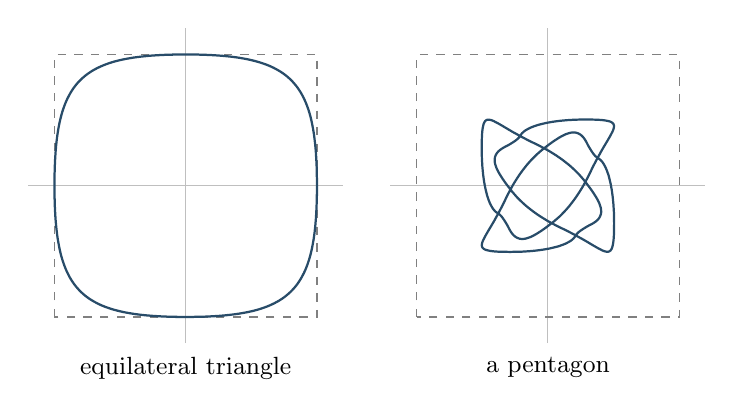
\begin{tikzpicture}
\begin{scope}[xshift=0.0cm]
\draw[gray!50] (-2,0) -- (2,0) (0,-2) -- (0,2);
\draw[gray,dashed] (-1.667,-1.667) rectangle (1.667,1.667);
\draw[inkblue,thick] (1.667,0.003) -- (1.666,0.106) -- (1.664,0.204) -- (1.661,0.296) -- (1.656,0.384) -- (1.650,0.466) -- (1.642,0.545) -- (1.633,0.619) -- (1.623,0.689) -- (1.611,0.756) -- (1.598,0.819) -- (1.584,0.879) -- (1.568,0.936) -- (1.550,0.990) -- (1.531,1.041) -- (1.510,1.090) -- (1.488,1.135) -- (1.464,1.179) -- (1.438,1.220) -- (1.410,1.259) -- (1.381,1.295) -- (1.350,1.330) -- (1.316,1.362) -- (1.281,1.393) -- (1.244,1.421) -- (1.204,1.448) -- (1.162,1.473) -- (1.118,1.497) -- (1.071,1.519) -- (1.021,1.539) -- (0.969,1.557) -- (0.914,1.574) -- (0.856,1.590) -- (0.795,1.604) -- (0.730,1.616) -- (0.662,1.627) -- (0.590,1.637) -- (0.514,1.645) -- (0.434,1.652) -- (0.350,1.658) -- (0.260,1.662) -- (0.166,1.665) -- (0.066,1.666) -- (-0.038,1.667) -- (-0.140,1.665) -- (-0.235,1.663) -- (-0.326,1.659) -- (-0.412,1.654) -- (-0.493,1.647) -- (-0.570,1.639) -- (-0.643,1.630) -- (-0.712,1.619) -- (-0.778,1.607) -- (-0.840,1.594) -- (-0.899,1.579) -- (-0.955,1.562) -- (-1.007,1.544) -- (-1.058,1.524) -- (-1.105,1.503) -- (-1.150,1.480) -- (-1.193,1.455) -- (-1.233,1.429) -- (-1.271,1.401) -- (-1.307,1.371) -- (-1.341,1.339) -- (-1.373,1.305) -- (-1.403,1.269) -- (-1.431,1.231) -- (-1.457,1.190) -- (-1.481,1.147) -- (-1.504,1.102) -- (-1.525,1.055) -- (-1.545,1.004) -- (-1.563,0.951) -- (-1.579,0.895) -- (-1.594,0.836) -- (-1.608,0.774) -- (-1.620,0.708) -- (-1.631,0.638) -- (-1.640,0.565) -- (-1.648,0.488) -- (-1.654,0.406) -- (-1.659,0.320) -- (-1.663,0.229) -- (-1.666,0.133) -- (-1.667,0.032) -- (-1.666,-0.073) -- (-1.665,-0.172) -- (-1.662,-0.266) -- (-1.657,-0.355) -- (-1.652,-0.439) -- (-1.645,-0.519) -- (-1.636,-0.595) -- (-1.627,-0.666) -- (-1.615,-0.734) -- (-1.603,-0.799) -- (-1.589,-0.860) -- (-1.573,-0.918) -- (-1.556,-0.973) -- (-1.537,-1.025) -- (-1.517,-1.074) -- (-1.495,-1.120) -- (-1.472,-1.165) -- (-1.447,-1.206) -- (-1.420,-1.246) -- (-1.391,-1.283) -- (-1.360,-1.318) -- (-1.328,-1.352) -- (-1.293,-1.383) -- (-1.256,-1.412) -- (-1.217,-1.440) -- (-1.176,-1.465) -- (-1.133,-1.489) -- (-1.087,-1.511) -- (-1.038,-1.532) -- (-0.987,-1.551) -- (-0.933,-1.569) -- (-0.876,-1.585) -- (-0.816,-1.599) -- (-0.752,-1.612) -- (-0.685,-1.624) -- (-0.614,-1.634) -- (-0.540,-1.643) -- (-0.461,-1.650) -- (-0.378,-1.656) -- (-0.291,-1.661) -- (-0.198,-1.664) -- (-0.100,-1.666) -- (0.003,-1.667) -- (0.106,-1.666) -- (0.204,-1.664) -- (0.296,-1.661) -- (0.384,-1.656) -- (0.466,-1.650) -- (0.545,-1.642) -- (0.619,-1.633) -- (0.689,-1.623) -- (0.756,-1.611) -- (0.819,-1.598) -- (0.879,-1.584) -- (0.936,-1.568) -- (0.990,-1.550) -- (1.041,-1.531) -- (1.090,-1.510) -- (1.135,-1.488) -- (1.179,-1.464) -- (1.220,-1.438) -- (1.259,-1.410) -- (1.295,-1.381) -- (1.330,-1.350) -- (1.362,-1.316) -- (1.393,-1.281) -- (1.421,-1.244) -- (1.448,-1.204) -- (1.473,-1.162) -- (1.497,-1.118) -- (1.519,-1.071) -- (1.539,-1.021) -- (1.557,-0.969) -- (1.574,-0.914) -- (1.590,-0.856) -- (1.604,-0.795) -- (1.616,-0.730) -- (1.627,-0.662) -- (1.637,-0.590) -- (1.645,-0.514) -- (1.652,-0.434) -- (1.658,-0.350) -- (1.662,-0.260) -- (1.665,-0.166) -- (1.666,-0.066) -- (1.667,0.038) -- (1.665,0.140) -- (1.663,0.235) -- (1.659,0.326) -- (1.654,0.412) -- (1.647,0.493) -- (1.639,0.570) -- (1.630,0.643) -- (1.619,0.712) -- (1.607,0.778) -- (1.594,0.840) -- (1.579,0.899) -- (1.562,0.955) -- (1.544,1.007) -- (1.524,1.058) -- (1.503,1.105) -- (1.480,1.150) -- (1.455,1.193) -- (1.429,1.233) -- (1.401,1.271) -- (1.371,1.307) -- (1.339,1.341) -- (1.305,1.373) -- (1.269,1.403) -- (1.231,1.431) -- (1.190,1.457) -- (1.147,1.481) -- (1.102,1.504) -- (1.055,1.525) -- (1.004,1.545) -- (0.951,1.563) -- (0.895,1.579) -- (0.836,1.594) -- (0.774,1.608) -- (0.708,1.620) -- (0.638,1.631) -- (0.565,1.640) -- (0.488,1.648) -- (0.406,1.654) -- (0.320,1.659) -- (0.229,1.663) -- (0.133,1.666) -- (0.032,1.667) -- (-0.073,1.666) -- (-0.172,1.665) -- (-0.266,1.662) -- (-0.355,1.657) -- (-0.439,1.652) -- (-0.519,1.645) -- (-0.595,1.636) -- (-0.666,1.627) -- (-0.734,1.615) -- (-0.799,1.603) -- (-0.860,1.589) -- (-0.918,1.573) -- (-0.973,1.556) -- (-1.025,1.537) -- (-1.074,1.517) -- (-1.120,1.495) -- (-1.165,1.472) -- (-1.206,1.447) -- (-1.246,1.420) -- (-1.283,1.391) -- (-1.318,1.360) -- (-1.352,1.328) -- (-1.383,1.293) -- (-1.412,1.256) -- (-1.440,1.217) -- (-1.465,1.176) -- (-1.489,1.133) -- (-1.511,1.087) -- (-1.532,1.038) -- (-1.551,0.987) -- (-1.569,0.933) -- (-1.585,0.876) -- (-1.599,0.816) -- (-1.612,0.752) -- (-1.624,0.685) -- (-1.634,0.614) -- (-1.643,0.540) -- (-1.650,0.461) -- (-1.656,0.378) -- (-1.661,0.291) -- (-1.664,0.198) -- (-1.666,0.100) -- (-1.667,-0.003) -- (-1.666,-0.106) -- (-1.664,-0.204) -- (-1.661,-0.296) -- (-1.656,-0.384) -- (-1.650,-0.466) -- (-1.642,-0.545) -- (-1.633,-0.619) -- (-1.623,-0.689) -- (-1.611,-0.756) -- (-1.598,-0.819) -- (-1.584,-0.879) -- (-1.568,-0.936) -- (-1.550,-0.990) -- (-1.531,-1.041) -- (-1.510,-1.090) -- (-1.488,-1.135) -- (-1.464,-1.179) -- (-1.438,-1.220) -- (-1.410,-1.259) -- (-1.381,-1.295) -- (-1.350,-1.330) -- (-1.316,-1.362) -- (-1.281,-1.393) -- (-1.244,-1.421) -- (-1.204,-1.448) -- (-1.162,-1.473) -- (-1.118,-1.497) -- (-1.071,-1.519) -- (-1.021,-1.539) -- (-0.969,-1.557) -- (-0.914,-1.574) -- (-0.856,-1.590) -- (-0.795,-1.604) -- (-0.730,-1.616) -- (-0.662,-1.627) -- (-0.590,-1.637) -- (-0.514,-1.645) -- (-0.434,-1.652) -- (-0.350,-1.658) -- (-0.260,-1.662) -- (-0.166,-1.665) -- (-0.066,-1.666) -- (0.038,-1.667) -- (0.140,-1.665) -- (0.235,-1.663) -- (0.326,-1.659) -- (0.412,-1.654) -- (0.493,-1.647) -- (0.570,-1.639) -- (0.643,-1.630) -- (0.712,-1.619) -- (0.778,-1.607) -- (0.840,-1.594) -- (0.899,-1.579) -- (0.955,-1.562) -- (1.007,-1.544) -- (1.058,-1.524) -- (1.105,-1.503) -- (1.150,-1.480) -- (1.193,-1.455) -- (1.233,-1.429) -- (1.271,-1.401) -- (1.307,-1.371) -- (1.341,-1.339) -- (1.373,-1.305) -- (1.403,-1.269) -- (1.431,-1.231) -- (1.457,-1.190) -- (1.481,-1.147) -- (1.504,-1.102) -- (1.525,-1.055) -- (1.545,-1.004) -- (1.563,-0.951) -- (1.579,-0.895) -- (1.594,-0.836) -- (1.608,-0.774) -- (1.620,-0.708) -- (1.631,-0.638) -- (1.640,-0.565) -- (1.648,-0.488) -- (1.654,-0.406) -- (1.659,-0.320) -- (1.663,-0.229) -- (1.666,-0.133) -- (1.667,-0.032) -- (1.666,0.073) -- (1.665,0.172) -- (1.662,0.266) -- (1.657,0.355) -- (1.652,0.439) -- (1.645,0.519) -- (1.636,0.595) -- (1.627,0.666) -- (1.615,0.734) -- (1.603,0.799) -- (1.589,0.860) -- (1.573,0.918) -- (1.556,0.973) -- (1.537,1.025) -- (1.517,1.074) -- (1.495,1.120) -- (1.472,1.165) -- (1.447,1.206) -- (1.420,1.246) -- (1.391,1.283) -- (1.360,1.318) -- (1.328,1.352) -- (1.293,1.383) -- (1.256,1.412) -- (1.217,1.440) -- (1.176,1.465) -- (1.133,1.489) -- (1.087,1.511) -- (1.038,1.532) -- (0.987,1.551) -- (0.933,1.569) -- (0.876,1.585) -- (0.816,1.599) -- (0.752,1.612) -- (0.685,1.624) -- (0.614,1.634) -- (0.540,1.643) -- (0.461,1.650) -- (0.378,1.656) -- (0.291,1.661) -- (0.198,1.664) -- (0.100,1.666) -- (-0.003,1.667) -- (-0.106,1.666) -- (-0.204,1.664) -- (-0.296,1.661) -- (-0.384,1.656) -- (-0.466,1.650) -- (-0.545,1.642) -- (-0.619,1.633) -- (-0.689,1.623) -- (-0.756,1.611) -- (-0.819,1.598) -- (-0.879,1.584) -- (-0.936,1.568) -- (-0.990,1.550) -- (-1.041,1.531) -- (-1.090,1.510) -- (-1.135,1.488) -- (-1.179,1.464) -- (-1.220,1.438) -- (-1.259,1.410) -- (-1.295,1.381) -- (-1.330,1.350) -- (-1.362,1.316) -- (-1.393,1.281) -- (-1.421,1.244) -- (-1.448,1.204) -- (-1.473,1.162) -- (-1.497,1.118) -- (-1.519,1.071) -- (-1.539,1.021) -- (-1.557,0.969) -- (-1.574,0.914) -- (-1.590,0.856) -- (-1.604,0.795) -- (-1.616,0.730) -- (-1.627,0.662) -- (-1.637,0.590) -- (-1.645,0.514) -- (-1.652,0.434) -- (-1.658,0.350) -- (-1.662,0.260) -- (-1.665,0.166) -- (-1.666,0.066) -- (-1.667,-0.038) -- (-1.665,-0.140) -- (-1.663,-0.235) -- (-1.659,-0.326) -- (-1.654,-0.412) -- (-1.647,-0.493) -- (-1.639,-0.570) -- (-1.630,-0.643) -- (-1.619,-0.712) -- (-1.607,-0.778) -- (-1.594,-0.840) -- (-1.579,-0.899) -- (-1.562,-0.955) -- (-1.544,-1.007) -- (-1.524,-1.058) -- (-1.503,-1.105) -- (-1.480,-1.150) -- (-1.455,-1.193) -- (-1.429,-1.233) -- (-1.401,-1.271) -- (-1.371,-1.307) -- (-1.339,-1.341) -- (-1.305,-1.373) -- (-1.269,-1.403) -- (-1.231,-1.431) -- (-1.190,-1.457) -- (-1.147,-1.481) -- (-1.102,-1.504) -- (-1.055,-1.525) -- (-1.004,-1.545) -- (-0.951,-1.563) -- (-0.895,-1.579) -- (-0.836,-1.594) -- (-0.774,-1.608) -- (-0.708,-1.620) -- (-0.638,-1.631) -- (-0.565,-1.640) -- (-0.488,-1.648) -- (-0.406,-1.654) -- (-0.320,-1.659) -- (-0.229,-1.663) -- (-0.133,-1.666) -- (-0.032,-1.667) -- (0.073,-1.666) -- (0.172,-1.665) -- (0.266,-1.662) -- (0.355,-1.657) -- (0.439,-1.652) -- (0.519,-1.645) -- (0.595,-1.636) -- (0.666,-1.627) -- (0.734,-1.615) -- (0.799,-1.603) -- (0.860,-1.589) -- (0.918,-1.573) -- (0.973,-1.556) -- (1.025,-1.537) -- (1.074,-1.517) -- (1.120,-1.495) -- (1.165,-1.472) -- (1.206,-1.447) -- (1.246,-1.420) -- (1.283,-1.391) -- (1.318,-1.360) -- (1.352,-1.328) -- (1.383,-1.293) -- (1.412,-1.256) -- (1.440,-1.217) -- (1.465,-1.176) -- (1.489,-1.133) -- (1.511,-1.087) -- (1.532,-1.038) -- (1.551,-0.987) -- (1.569,-0.933) -- (1.585,-0.876) -- (1.599,-0.816) -- (1.612,-0.752) -- (1.624,-0.685) -- (1.634,-0.614) -- (1.643,-0.540) -- (1.650,-0.461) -- (1.656,-0.378) -- (1.661,-0.291) -- (1.664,-0.198) -- (1.666,-0.100) -- cycle;
\node[below] at (0,-2.05) {\small equilateral triangle};
\end{scope}
\begin{scope}[xshift=4.6cm]
\draw[gray!50] (-2,0) -- (2,0) (0,-2) -- (0,2);
\draw[gray,dashed] (-1.667,-1.667) rectangle (1.667,1.667);
\draw[inkblue,thick] (0.567,0.420) -- (0.553,0.441) -- (0.538,0.465) -- (0.522,0.491) -- (0.506,0.520) -- (0.490,0.552) -- (0.473,0.581) -- (0.456,0.606) -- (0.438,0.627) -- (0.419,0.644) -- (0.400,0.657) -- (0.380,0.666) -- (0.360,0.673) -- (0.339,0.676) -- (0.317,0.676) -- (0.294,0.674) -- (0.271,0.669) -- (0.247,0.661) -- (0.222,0.652) -- (0.197,0.640) -- (0.170,0.626) -- (0.142,0.610) -- (0.114,0.592) -- (0.084,0.573) -- (0.054,0.552) -- (0.022,0.529) -- (-0.011,0.504) -- (-0.045,0.478) -- (-0.079,0.451) -- (-0.113,0.422) -- (-0.147,0.392) -- (-0.179,0.360) -- (-0.211,0.327) -- (-0.242,0.293) -- (-0.272,0.258) -- (-0.301,0.221) -- (-0.330,0.183) -- (-0.358,0.144) -- (-0.385,0.104) -- (-0.411,0.063) -- (-0.437,0.021) -- (-0.462,-0.023) -- (-0.486,-0.068) -- (-0.510,-0.113) -- (-0.533,-0.160) -- (-0.555,-0.206) -- (-0.576,-0.249) -- (-0.597,-0.289) -- (-0.617,-0.327) -- (-0.636,-0.363) -- (-0.655,-0.396) -- (-0.672,-0.428) -- (-0.689,-0.458) -- (-0.705,-0.485) -- (-0.721,-0.512) -- (-0.735,-0.536) -- (-0.749,-0.559) -- (-0.762,-0.581) -- (-0.774,-0.602) -- (-0.785,-0.621) -- (-0.795,-0.639) -- (-0.804,-0.656) -- (-0.812,-0.672) -- (-0.820,-0.687) -- (-0.826,-0.701) -- (-0.831,-0.714) -- (-0.835,-0.727) -- (-0.837,-0.738) -- (-0.839,-0.749) -- (-0.839,-0.759) -- (-0.838,-0.768) -- (-0.835,-0.777) -- (-0.831,-0.785) -- (-0.825,-0.792) -- (-0.818,-0.799) -- (-0.809,-0.805) -- (-0.798,-0.811) -- (-0.785,-0.816) -- (-0.770,-0.820) -- (-0.752,-0.824) -- (-0.733,-0.828) -- (-0.711,-0.831) -- (-0.686,-0.834) -- (-0.658,-0.836) -- (-0.627,-0.838) -- (-0.593,-0.839) -- (-0.556,-0.840) -- (-0.518,-0.840) -- (-0.480,-0.841) -- (-0.444,-0.840) -- (-0.408,-0.840) -- (-0.372,-0.839) -- (-0.337,-0.838) -- (-0.303,-0.836) -- (-0.270,-0.834) -- (-0.237,-0.832) -- (-0.205,-0.829) -- (-0.174,-0.826) -- (-0.143,-0.823) -- (-0.113,-0.819) -- (-0.083,-0.815) -- (-0.055,-0.811) -- (-0.027,-0.806) -- (0.000,-0.801) -- (0.027,-0.796) -- (0.052,-0.790) -- (0.077,-0.784) -- (0.101,-0.778) -- (0.125,-0.772) -- (0.147,-0.765) -- (0.169,-0.757) -- (0.189,-0.750) -- (0.209,-0.742) -- (0.228,-0.734) -- (0.245,-0.725) -- (0.262,-0.716) -- (0.278,-0.707) -- (0.292,-0.698) -- (0.305,-0.688) -- (0.317,-0.677) -- (0.328,-0.667) -- (0.337,-0.656) -- (0.345,-0.644) -- (0.352,-0.632) -- (0.361,-0.620) -- (0.372,-0.607) -- (0.385,-0.594) -- (0.401,-0.581) -- (0.420,-0.567) -- (0.441,-0.553) -- (0.465,-0.538) -- (0.491,-0.522) -- (0.520,-0.506) -- (0.552,-0.490) -- (0.581,-0.473) -- (0.606,-0.456) -- (0.627,-0.438) -- (0.644,-0.419) -- (0.657,-0.400) -- (0.666,-0.380) -- (0.673,-0.360) -- (0.676,-0.339) -- (0.676,-0.317) -- (0.674,-0.294) -- (0.669,-0.271) -- (0.661,-0.247) -- (0.652,-0.222) -- (0.640,-0.197) -- (0.626,-0.170) -- (0.610,-0.142) -- (0.592,-0.114) -- (0.573,-0.084) -- (0.552,-0.054) -- (0.529,-0.022) -- (0.504,0.011) -- (0.478,0.045) -- (0.451,0.079) -- (0.422,0.113) -- (0.392,0.147) -- (0.360,0.179) -- (0.327,0.211) -- (0.293,0.242) -- (0.258,0.272) -- (0.221,0.301) -- (0.183,0.330) -- (0.144,0.358) -- (0.104,0.385) -- (0.063,0.411) -- (0.021,0.437) -- (-0.023,0.462) -- (-0.068,0.486) -- (-0.113,0.510) -- (-0.160,0.533) -- (-0.206,0.555) -- (-0.249,0.576) -- (-0.289,0.597) -- (-0.327,0.617) -- (-0.363,0.636) -- (-0.396,0.655) -- (-0.428,0.672) -- (-0.458,0.689) -- (-0.485,0.705) -- (-0.512,0.721) -- (-0.536,0.735) -- (-0.559,0.749) -- (-0.581,0.762) -- (-0.602,0.774) -- (-0.621,0.785) -- (-0.639,0.795) -- (-0.656,0.804) -- (-0.672,0.812) -- (-0.687,0.820) -- (-0.701,0.826) -- (-0.714,0.831) -- (-0.727,0.835) -- (-0.738,0.837) -- (-0.749,0.839) -- (-0.759,0.839) -- (-0.768,0.838) -- (-0.777,0.835) -- (-0.785,0.831) -- (-0.792,0.825) -- (-0.799,0.818) -- (-0.805,0.809) -- (-0.811,0.798) -- (-0.816,0.785) -- (-0.820,0.770) -- (-0.824,0.752) -- (-0.828,0.733) -- (-0.831,0.711) -- (-0.834,0.686) -- (-0.836,0.658) -- (-0.838,0.627) -- (-0.839,0.593) -- (-0.840,0.556) -- (-0.840,0.518) -- (-0.841,0.480) -- (-0.840,0.444) -- (-0.840,0.408) -- (-0.839,0.372) -- (-0.838,0.337) -- (-0.836,0.303) -- (-0.834,0.270) -- (-0.832,0.237) -- (-0.829,0.205) -- (-0.826,0.174) -- (-0.823,0.143) -- (-0.819,0.113) -- (-0.815,0.083) -- (-0.811,0.055) -- (-0.806,0.027) -- (-0.801,-0.000) -- (-0.796,-0.027) -- (-0.790,-0.052) -- (-0.784,-0.077) -- (-0.778,-0.101) -- (-0.772,-0.125) -- (-0.765,-0.147) -- (-0.757,-0.169) -- (-0.750,-0.189) -- (-0.742,-0.209) -- (-0.734,-0.228) -- (-0.725,-0.245) -- (-0.716,-0.262) -- (-0.707,-0.278) -- (-0.698,-0.292) -- (-0.688,-0.305) -- (-0.677,-0.317) -- (-0.667,-0.328) -- (-0.656,-0.337) -- (-0.644,-0.345) -- (-0.632,-0.352) -- (-0.620,-0.361) -- (-0.607,-0.372) -- (-0.594,-0.385) -- (-0.581,-0.401) -- (-0.567,-0.420) -- (-0.553,-0.441) -- (-0.538,-0.465) -- (-0.522,-0.491) -- (-0.506,-0.520) -- (-0.490,-0.552) -- (-0.473,-0.581) -- (-0.456,-0.606) -- (-0.438,-0.627) -- (-0.419,-0.644) -- (-0.400,-0.657) -- (-0.380,-0.666) -- (-0.360,-0.673) -- (-0.339,-0.676) -- (-0.317,-0.676) -- (-0.294,-0.674) -- (-0.271,-0.669) -- (-0.247,-0.661) -- (-0.222,-0.652) -- (-0.197,-0.640) -- (-0.170,-0.626) -- (-0.142,-0.610) -- (-0.114,-0.592) -- (-0.084,-0.573) -- (-0.054,-0.552) -- (-0.022,-0.529) -- (0.011,-0.504) -- (0.045,-0.478) -- (0.079,-0.451) -- (0.113,-0.422) -- (0.147,-0.392) -- (0.179,-0.360) -- (0.211,-0.327) -- (0.242,-0.293) -- (0.272,-0.258) -- (0.301,-0.221) -- (0.330,-0.183) -- (0.358,-0.144) -- (0.385,-0.104) -- (0.411,-0.063) -- (0.437,-0.021) -- (0.462,0.023) -- (0.486,0.068) -- (0.510,0.113) -- (0.533,0.160) -- (0.555,0.206) -- (0.576,0.249) -- (0.597,0.289) -- (0.617,0.327) -- (0.636,0.363) -- (0.655,0.396) -- (0.672,0.428) -- (0.689,0.458) -- (0.705,0.485) -- (0.721,0.512) -- (0.735,0.536) -- (0.749,0.559) -- (0.762,0.581) -- (0.774,0.602) -- (0.785,0.621) -- (0.795,0.639) -- (0.804,0.656) -- (0.812,0.672) -- (0.820,0.687) -- (0.826,0.701) -- (0.831,0.714) -- (0.835,0.727) -- (0.837,0.738) -- (0.839,0.749) -- (0.839,0.759) -- (0.838,0.768) -- (0.835,0.777) -- (0.831,0.785) -- (0.825,0.792) -- (0.818,0.799) -- (0.809,0.805) -- (0.798,0.811) -- (0.785,0.816) -- (0.770,0.820) -- (0.752,0.824) -- (0.733,0.828) -- (0.711,0.831) -- (0.686,0.834) -- (0.658,0.836) -- (0.627,0.838) -- (0.593,0.839) -- (0.556,0.840) -- (0.518,0.840) -- (0.480,0.841) -- (0.444,0.840) -- (0.408,0.840) -- (0.372,0.839) -- (0.337,0.838) -- (0.303,0.836) -- (0.270,0.834) -- (0.237,0.832) -- (0.205,0.829) -- (0.174,0.826) -- (0.143,0.823) -- (0.113,0.819) -- (0.083,0.815) -- (0.055,0.811) -- (0.027,0.806) -- (-0.000,0.801) -- (-0.027,0.796) -- (-0.052,0.790) -- (-0.077,0.784) -- (-0.101,0.778) -- (-0.125,0.772) -- (-0.147,0.765) -- (-0.169,0.757) -- (-0.189,0.750) -- (-0.209,0.742) -- (-0.228,0.734) -- (-0.245,0.725) -- (-0.262,0.716) -- (-0.278,0.707) -- (-0.292,0.698) -- (-0.305,0.688) -- (-0.317,0.677) -- (-0.328,0.667) -- (-0.337,0.656) -- (-0.345,0.644) -- (-0.352,0.632) -- (-0.361,0.620) -- (-0.372,0.607) -- (-0.385,0.594) -- (-0.401,0.581) -- (-0.420,0.567) -- (-0.441,0.553) -- (-0.465,0.538) -- (-0.491,0.522) -- (-0.520,0.506) -- (-0.552,0.490) -- (-0.581,0.473) -- (-0.606,0.456) -- (-0.627,0.438) -- (-0.644,0.419) -- (-0.657,0.400) -- (-0.666,0.380) -- (-0.673,0.360) -- (-0.676,0.339) -- (-0.676,0.317) -- (-0.674,0.294) -- (-0.669,0.271) -- (-0.661,0.247) -- (-0.652,0.222) -- (-0.640,0.197) -- (-0.626,0.170) -- (-0.610,0.142) -- (-0.592,0.114) -- (-0.573,0.084) -- (-0.552,0.054) -- (-0.529,0.022) -- (-0.504,-0.011) -- (-0.478,-0.045) -- (-0.451,-0.079) -- (-0.422,-0.113) -- (-0.392,-0.147) -- (-0.360,-0.179) -- (-0.327,-0.211) -- (-0.293,-0.242) -- (-0.258,-0.272) -- (-0.221,-0.301) -- (-0.183,-0.330) -- (-0.144,-0.358) -- (-0.104,-0.385) -- (-0.063,-0.411) -- (-0.021,-0.437) -- (0.023,-0.462) -- (0.068,-0.486) -- (0.113,-0.510) -- (0.160,-0.533) -- (0.206,-0.555) -- (0.249,-0.576) -- (0.289,-0.597) -- (0.327,-0.617) -- (0.363,-0.636) -- (0.396,-0.655) -- (0.428,-0.672) -- (0.458,-0.689) -- (0.485,-0.705) -- (0.512,-0.721) -- (0.536,-0.735) -- (0.559,-0.749) -- (0.581,-0.762) -- (0.602,-0.774) -- (0.621,-0.785) -- (0.639,-0.795) -- (0.656,-0.804) -- (0.672,-0.812) -- (0.687,-0.820) -- (0.701,-0.826) -- (0.714,-0.831) -- (0.727,-0.835) -- (0.738,-0.837) -- (0.749,-0.839) -- (0.759,-0.839) -- (0.768,-0.838) -- (0.777,-0.835) -- (0.785,-0.831) -- (0.792,-0.825) -- (0.799,-0.818) -- (0.805,-0.809) -- (0.811,-0.798) -- (0.816,-0.785) -- (0.820,-0.770) -- (0.824,-0.752) -- (0.828,-0.733) -- (0.831,-0.711) -- (0.834,-0.686) -- (0.836,-0.658) -- (0.838,-0.627) -- (0.839,-0.593) -- (0.840,-0.556) -- (0.840,-0.518) -- (0.841,-0.480) -- (0.840,-0.444) -- (0.840,-0.408) -- (0.839,-0.372) -- (0.838,-0.337) -- (0.836,-0.303) -- (0.834,-0.270) -- (0.832,-0.237) -- (0.829,-0.205) -- (0.826,-0.174) -- (0.823,-0.143) -- (0.819,-0.113) -- (0.815,-0.083) -- (0.811,-0.055) -- (0.806,-0.027) -- (0.801,0.000) -- (0.796,0.027) -- (0.790,0.052) -- (0.784,0.077) -- (0.778,0.101) -- (0.772,0.125) -- (0.765,0.147) -- (0.757,0.169) -- (0.750,0.189) -- (0.742,0.209) -- (0.734,0.228) -- (0.725,0.245) -- (0.716,0.262) -- (0.707,0.278) -- (0.698,0.292) -- (0.688,0.305) -- (0.677,0.317) -- (0.667,0.328) -- (0.656,0.337) -- (0.644,0.345) -- (0.632,0.352) -- (0.620,0.361) -- (0.607,0.372) -- (0.594,0.385) -- (0.581,0.401) -- cycle;
\node[below] at (0,-2.05) {\small a pentagon};
\end{scope}
\end{tikzpicture}

\caption{The curve $\theta\mapsto(b(\theta),b(\theta+\pi/2))$, drawn to the same scale for an
equilateral triangle and for the pentagon with vertices $(0,0)$, $(3,0)$, $(3.5,1)$, $(1,2.2)$,
$(-0.4,1)$. The dashed square is $\abs{x},\abs{y}\le 1/18$. By~\eqref{eq:area}, $P(K)-\tfrac12$ is half
the area enclosed, counted with multiplicity: about $0.0164$ for the triangle, run round three times,
and $0.0024$ for the pentagon.}
\label{fig:curve}
\end{figure}

\begin{remark}
If $\gamma$ avoids the origin, its winding number about the origin is $\equiv 3 \pmod 4$, because each
quarter of the parameter turns $\gamma$ through a quarter turn clockwise plus a whole number of full
turns. A winding number of $3$ needs at least three lines through $G$ that halve the area of $K$. This
remark is not used below.
\end{remark}

\section{How symmetric is \texorpdfstring{$K$}{K}?}\label{sec:sym}

Proposition~\ref{prop:key} has two factors, and each measures how far $K$ is from being symmetric about
$G$. The factor $b$ is the imbalance of a line through $G$. Write $g(K)$ for its largest value
$\max_\theta\abs{b(\theta)}$, the worst imbalance of a line through the centroid.

The factor $\ro$ has a meaning of its own once it is integrated. For positive $x$ and $y$,
$\tfrac12\abs{x-y}=\tfrac12(x+y)-\min(x,y)$, and $\tfrac12\min\bigl(r(\theta),r(\theta+\pi)\bigr)^2$ is
the area element of $K\cap(-K)$, the largest part of $K$ that is symmetric about $G$. So
\begin{equation}\label{eq:sym}
\int_0^{2\pi}\abs{\ro(\theta)}\,d\theta = 1-s(K),\qquad s(K)=\frac{\abs{K\cap(-K)}}{\abs{K}} ,
\end{equation}
where $s(K)$ is the share of $K$ that is centrally symmetric about the centroid. Bounding $b$ by $g(K)$
in Proposition~\ref{prop:key} and using~\eqref{eq:sym} gives the estimate behind Theorem~\ref{thm:A}.

\begin{proposition}\label{prop:product}
$\abs{P(K)-\tfrac12}\le g(K)\,\bigl(1-s(K)\bigr)$.
\end{proposition}

Both factors have known worst cases, and in both the worst case is a triangle.

\emph{Gr\"unbaum's inequality}~\cite[Theorem~2 and its proof]{Gru60}: every line through the centroid of
a planar convex region leaves at least $4/9$ of the area on each side. Equality holds for a triangle cut
by the line through $G$ parallel to a side. So $g(K)\le 1/18$.

\emph{Stewart's inequality}~\cite{Ste58}: for every planar convex region,
$\abs{K\cap(2G-K)}\ge\tfrac23\abs{K}$, that is, $s(K)\ge 2/3$. For a triangle, $K\cap(-K)$ is the hexagon
cut out by the triangle and its reflection (Figure~\ref{fig:hexagon}), which has exactly two thirds of
the area.

\begin{proof}[Proof of Theorem~\ref{thm:A}]
Put the two inequalities into Proposition~\ref{prop:product}:
$\abs{P(K)-\tfrac12}\le\tfrac1{18}\cdot\tfrac13=\tfrac1{54}$.
\end{proof}

Stewart's inequality sits in a longer history. Kovner, and independently Besicovitch~\cite{Bes48} and
Fáry, proved that every planar convex region contains a centrally symmetric convex region with at least
two thirds of its area (for this history see~\cite{Fel26}). There the centre of symmetry is chosen to
suit $K$. Fáry and Rédei showed that for a simplex the best centre is the centroid~\cite[Satz~5]{FR50}.
At the centroid itself the first general bound was Levi's~\cite{Lev52}, as reported by
Stein~\cite[Theorem~3]{Ste56}. It follows from the Minkowski--Radon inequality, that the centroid divides
every chord through it in a ratio at most $2:1$ (see~\cite[Section~2]{Fel26}). Then
$\rho(\theta)\le4\rho(\theta+\pi)$, and if $x\le 4y$ and $y\le 4x$ then $\abs{x-y}\le\tfrac35(x+y)$, so
$\int\abs{\ro}\le\tfrac35$ and $s(K)\ge 2/5$. With Gr\"unbaum's inequality this already gives
$P(K)\le\tfrac12+\tfrac1{18}\cdot\tfrac35=\tfrac8{15}$. Stewart's proof that $2/5$ can be raised to $2/3$
works cap by cap: each piece of $K$ outside $-K$ has at most the area of the triangle formed by $G$ and
the two ends of that piece, and the centroid condition, through a comparison of moments, is what
forbids more.

Both inequalities are equalities for every triangle, as $g$ and $s$ are unchanged by affine maps, so
Proposition~\ref{prop:product} gives exactly $14/27$ for every triangle while $P$ itself varies.
Table~\ref{tab:values} compares the bound with the true value for a few regions.

\begin{figure}[ht]
\centering
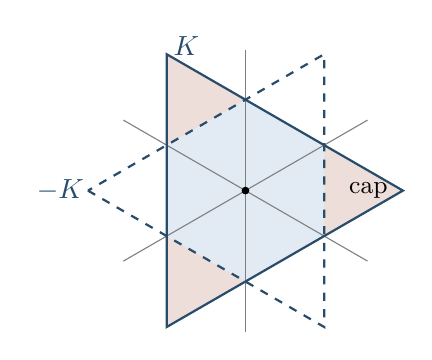
\begin{tikzpicture}
\draw[fill=rust!18,draw=none] (2.0000,0.0000) -- (-1.0000,1.7321) -- (-1.0000,-1.7321) -- cycle;
\draw[fill=softblue,draw=none] (-1.0000,-0.5774) -- (-0.0000,-1.1547) -- (1.0000,-0.5774) -- (1.0000,0.5774) -- (0.0000,1.1547) -- (-1.0000,0.5774) -- cycle;
\draw[gray] (1.550,0.895) -- (-1.550,-0.895);
\draw[gray] (0.000,1.790) -- (-0.000,-1.790);
\draw[gray] (-1.550,0.895) -- (1.550,-0.895);
\draw[thick,inkblue] (2.0000,0.0000) -- (-1.0000,1.7321) -- (-1.0000,-1.7321) -- cycle;
\draw[thick,inkblue,dashed] (-2.0000,-0.0000) -- (1.0000,-1.7321) -- (1.0000,1.7321) -- cycle;
\fill (0,0) circle (1.4pt);
\node at (1.560,0.000) {\small cap};
\node[inkblue] at (-0.750,1.832) {$K$};
\node[inkblue] at (-2.350,-0.000) {$-K$};
\end{tikzpicture}

\caption{An equilateral triangle $K$ and its reflection $-K$ through the centroid (dashed). Their
common part is the hexagon $K\cap(-K)$, with $2/3$ of the area; the three caps hold the rest. The three
lines through the centroid pass through opposite crossing points of the two boundaries. They cut the
plane into six sectors, and the caps lie in alternate sectors.}
\label{fig:hexagon}
\end{figure}

\begin{table}[ht]
\centering
\begin{tabular}{lcccc}
\toprule
region & $P(K)$ & $g(K)$ & $s(K)$ & $\tfrac12+g(K)(1-s(K))$\\
\midrule
square & $0.500000$ & $0$ & $1$ & $0.500000$\\
regular pentagon & $0.499054$ & $0.010557$ & $0.894427$ & $0.501115$\\
half-disc & $0.501321$ & $0.034468$ & $0.814753$ & $0.506385$\\
triangle with sides $3,4,5$ & $0.506629$ & $1/18$ & $2/3$ & $14/27$\\
right isosceles triangle & $0.509825$ & $1/18$ & $2/3$ & $14/27$\\
triangle $(0,0),(1,0),(0.2,0.7)$ & $0.510138$ & $1/18$ & $2/3$ & $14/27$\\
equilateral triangle & $0.516435$ & $1/18$ & $2/3$ & $14/27$\\
\bottomrule
\end{tabular}
\caption{The bound of Proposition~\ref{prop:product} against the true value. The bound is the same for
every triangle, because $g$ and $s$ are unchanged by affine maps; $P$ is not, which is where the gap
between $14/27\approx 0.518519$ and $0.516435$ comes from. Values to six decimals; the half-disc is
approximated by a $3000$-gon.}
\label{tab:values}
\end{table}

\section{A short proof near triangles}\label{sec:near}

For regions close to a triangle, Stewart's inequality follows from Gr\"unbaum's in three lines. The
reflection $-K$ has the same centroid as $K$, and the direction $\theta$ belongs to a cap of $K$ (a piece
of $K$ outside $-K$) exactly when $r(\theta)>r(\theta+\pi)$. Say that $K$ is \emph{three-sided} if there
are three lines through $G$ such that, in the six sectors they cut out, $r(\theta)\ge r(\theta+\pi)$ in
alternate sectors and $r(\theta)\le r(\theta+\pi)$ in the others. This is what it means for the two
boundaries to cross six times: the lines are the ones through opposite crossing points, as in
Figure~\ref{fig:hexagon}.

\begin{lemma}\label{lem:three}
Three lines through the centroid of a convex region $K$ cut it into six sectors. The three alternate
sectors together hold at most $2/3$ of the area of $K$.
\end{lemma}

\begin{proof}
Number the sectors $S_1,\dots,S_6$ in order round $G$, and take the half-plane bounded by each line that
contains $S_1S_2S_3$, $S_3S_4S_5$ and $S_5S_6S_1$ respectively. By Gr\"unbaum's inequality each holds at
most $5/9$ of the area. Together they cover $S_1$, $S_3$ and $S_5$ twice and the other sectors once, so
$\abs{K}+\abs{K\cap(S_1\cup S_3\cup S_5)}\le\tfrac{15}9\abs{K}$.
\end{proof}

\begin{proposition}\label{prop:near}
If $K$ is three-sided, then $s(K)\ge 2/3$.
\end{proposition}

\begin{proof}
Let $O$ be the union of the three sectors in which $r(\theta)\ge r(\theta+\pi)$. Then $\abs{\ro}=\ro$ on
$O$ and $\abs{\ro}=-\ro$ on its reflection, which is the rest of the plane, so
$\int\abs{\ro}=2\int_O\ro=\mu(O)-\mu(-O)=2\mu(O)-1$, where $\mu$ is the share of the area of $K$. By
Lemma~\ref{lem:three}, $\mu(O)\le 2/3$, so $1-s(K)\le 1/3$ by~\eqref{eq:sym}.
\end{proof}

\begin{remark}
Every convex region close enough to a triangle in the Hausdorff metric is three-sided. Here is the
reason, given as a sketch. A triangle and its reflection cross transversally at six points and are
well apart elsewhere. Near a transversal crossing, two convex curves that are uniformly close to two
lines of different slopes have one-sided slopes close to those of the lines, so they cross exactly once
there. Of $3000$ random convex polygons (convex hulls of $5$ to $10$ random points), $2550$ were three-sided.
For the others the boundaries cross ten or more times, and Lemma~\ref{lem:three} alone does not suffice:
an angular density with five caps of $1/9$ each, alternating with their reflections in ten arcs of
$36^\circ$, satisfies Gr\"unbaum's inequality and the Minkowski--Radon inequality in every direction and
has $s=4/9$. It is not the density of a convex region, which is why Stewart's proof uses convexity cap by
cap.
\end{remark}

\section{What is left}\label{sec:left}

\paragraph{The sharp bound.} The conjecture from the original question is that
$P(K)\le\tfrac13+\tfrac16\ln 3$, with equality only for equilateral triangles. Two numerical facts
support it. A local search for the maximum of $P$ over convex polygons with three to eight vertices,
started from $36$ random shapes, ended at the equilateral triangle $35$ times; the other run drifted
towards a segment, where $P$ is close to $1/2$. And allowing the marked point to be any interior point
of a polygon with up to six vertices does not help: the best found is still the equilateral triangle
with its centroid marked.

Proposition~\ref{prop:product} cannot reach the sharp value, because both of its factors are affine
invariants and every triangle gives the same bound. The usual route to such results is also closed.
Moving each vertex of a polygon along one fixed direction at its own constant speed (a shadow system,
after Shephard~\cite{She64}) keeps many functionals of random points convex, and that
forces their maxima onto triangles. Here $P$ is not even quasi-convex along shadow systems, already
within the family of triangles, since the equilateral triangle beats its affine images. A sharp proof
would have to use $b(\theta)$ and $b(\theta+\pi/2)$ together, as the area formula~\eqref{eq:area}
suggests, and not each separately.

\paragraph{Verification.} Propositions~\ref{prop:key} and~\ref{prop:product}, formula~\eqref{eq:area},
Lemma~\ref{lem:three}, Proposition~\ref{prop:near}, Theorem~\ref{thm:A} and the bound $8/15$ are
formalised in Lean~4 with Mathlib~\cite{mathlib}, using only the standard axioms, for densities $\rho$
that are continuous, $2\pi$-periodic and of total mass $1$. The inputs taken from the literature are
stated there as hypotheses (the inequalities of Gr\"unbaum, Stewart, and Minkowski and Radon), and
formula~\eqref{eq:P} is the definition of $P$ there. Stewart's cap-by-cap inequality was also checked
numerically on $1500$ random polygons. Python programs compute $P$, $g$ and $s$ exactly for polygons, check the
identities on examples, reproduce Table~\ref{tab:values} and the asker's values, and run the searches
quoted in Section~\ref{sec:left}. An independent program, sharing no code with them, rechecks the
table and the stated values by Monte Carlo and by direct geometry. Everything is at
\url{https://github.com/jvvk/mathematics/tree/main/catching-the-centroid}.

\paragraph{Acknowledgements.} Dan asked the question; Ethan Bolker, Franklin Pezzuti Dyer, Marco and
David~K answered it on Mathematics Stack Exchange, and Marco's Fourier series for regular polygons is
close in spirit to Proposition~\ref{prop:key}. Anthropic's Claude (Opus~5.5) was used to find the
arguments, write the Lean formalisation and the checking programs, and draft this text. The author
takes responsibility for the content.

\begin{thebibliography}{10}
\bibitem{MSE} Dan, What planar convex shape maximizes the probability that a random circle contains the
centre? (Surprisingly, it's not a disk.), Mathematics Stack Exchange question 5101873 (14 October 2025),
\url{https://math.stackexchange.com/q/5101873}, accessed 10 October 2026.
\bibitem{Bes48} A.~S.~Besicovitch, Measure of asymmetry of convex curves, \emph{J. London Math. Soc.}
\textbf{23} (1948) 237--240, \href{https://doi.org/10.1112/jlms/s1-23.3.237}{doi:10.1112/jlms/s1-23.3.237}.
\bibitem{FR50} I.~F\'ary and L.~R\'edei, Der zentralsymmetrische Kern und die zentralsymmetrische H\"ulle
von konvexen K\"orpern, \emph{Math. Ann.} \textbf{122} (1950) 205--220,
\href{https://doi.org/10.1007/BF01342966}{doi:10.1007/BF01342966}.
\bibitem{Fel26} D.~V.~Feldman, Arranging convex bodies for maximum intersection volume: the sharp
efficiency of centroid alignment, arXiv:2608.04516 (2026).
\bibitem{Gru60} B.~Gr\"unbaum, Partitions of mass-distributions and of convex bodies by hyperplanes,
\emph{Pacific J. Math.} \textbf{10} (1960) 1257--1261,
\href{https://doi.org/10.2140/pjm.1960.10.1257}{doi:10.2140/pjm.1960.10.1257}.
\bibitem{Lev52} F.~W.~Levi, \"Uber zwei S\"atze von Herrn Besicovitch, \emph{Arch. Math.} \textbf{3}
(1952) 125--129, \href{https://doi.org/10.1007/BF01899353}{doi:10.1007/BF01899353}.
\bibitem{Ste56} S.~Stein, The symmetry function in a convex body, \emph{Pacific J. Math.} \textbf{6}
(1956) 145--148, \href{https://doi.org/10.2140/pjm.1956.6.145}{doi:10.2140/pjm.1956.6.145}.
\bibitem{Ste58} B.~M.~Stewart, Asymmetry of a plane convex set with respect to its centroid,
\emph{Pacific J. Math.} \textbf{8} (1958) 335--337,
\href{https://doi.org/10.2140/pjm.1958.8.335}{doi:10.2140/pjm.1958.8.335}.
\bibitem{She64} G.~C.~Shephard, Shadow systems of convex sets, \emph{Israel J. Math.} \textbf{2} (1964)
229--236, \href{https://doi.org/10.1007/BF02759738}{doi:10.1007/BF02759738}.
\bibitem{mathlib} The mathlib Community, The Lean mathematical library, in \emph{Proceedings of the
9th ACM SIGPLAN International Conference on Certified Programs and Proofs (CPP 2020)}, 367--381,
\href{https://doi.org/10.1145/3372885.3373824}{doi:10.1145/3372885.3373824}.
\end{thebibliography}

\bigskip
\noindent Vamshi Jandhyala, London, UK.

\end{document}
